% Detailed methodology and architecture
\section{System Architecture \& Methodology}

\subsection{System Architecture}
The supplied block diagram is an earlier revision: it shows one Arduino and a direct UART link, while the project owner has confirmed front and rear Arduino Nano nodes on a shared USB-RS-485 bus, each controlling two motors. Until the editable source and PNG are updated, treat the figure as a preliminary artifact that does not represent the current controller topology.

\IfFileExists{figures/block_diagram.pdf}{
    \begin{figure}[!htbp]
        \centering
        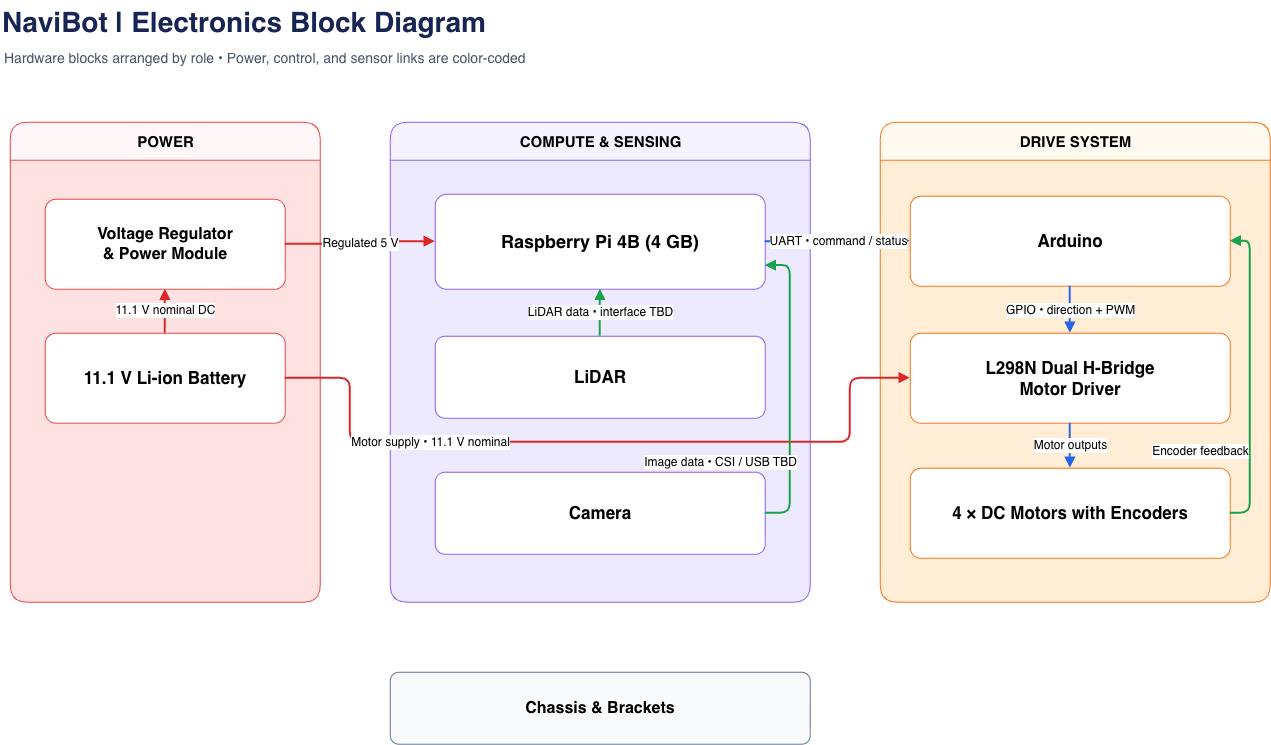
\includegraphics[width=0.92\textwidth,height=0.58\textheight,keepaspectratio]{figures/block_diagram}
        \caption{NaviBot electronics block diagram.}
        \label{fig:block_diagram}
    \end{figure}
}{\IfFileExists{figures/block_diagram.png}{
    \begin{figure}[!htbp]
        \centering
        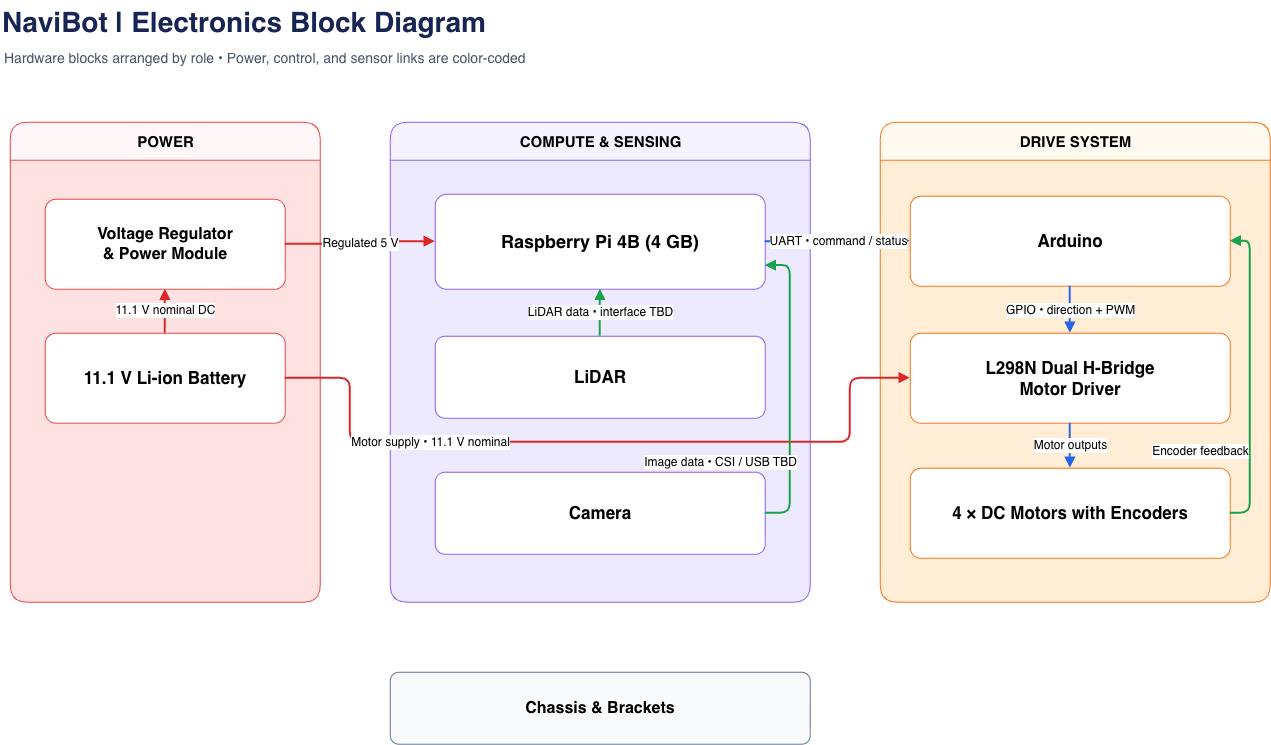
\includegraphics[width=0.92\textwidth,height=0.58\textheight,keepaspectratio]{figures/block_diagram}
        \caption{NaviBot electronics block diagram.}
        \label{fig:block_diagram}
    \end{figure}
}{}}

\subsection{Hardware and Electrical Design}
The block diagram labels a nominal 11.1 V battery supply, a voltage-regulator/power module, Pi and Arduino controllers, sensors, an L298N motor driver, and four encoder-equipped DC motors. Detailed schematics, part numbers, rail requirements, current budgets, protection, wiring, and grounding are TBD. Confirm that the selected driver and supply are suitable for the chosen motors before treating this architecture as final.

\IfFileExists{figures/circuit_diagram.pdf}{
    \begin{figure}[!htbp]
        \centering
        \includegraphics[width=0.95\textwidth,height=0.62\textheight,keepaspectratio]{figures/circuit_diagram}
        \caption{NaviBot circuit diagram.}
        \label{fig:circuit_diagram}
    \end{figure}
}{\IfFileExists{figures/circuit_diagram.png}{
    \begin{figure}[!htbp]
        \centering
        \includegraphics[width=0.95\textwidth,height=0.62\textheight,keepaspectratio]{figures/circuit_diagram}
        \caption{NaviBot circuit diagram.}
        \label{fig:circuit_diagram}
    \end{figure}
}{\textit{Circuit-level schematic not yet supplied.}}}

\subsection{Subsystem Configuration}
\subsubsection{Compute and Sensing}
The diagram depicts a Raspberry Pi 4B (4 GB), LiDAR, and camera, connected to an Arduino by UART. The confirmed design uses a USB-RS-485 adapter at the Pi and a shared bus with front and rear Arduino Nano nodes; the camera model is Pi Camera V2 (IMX219), and the serial LiDAR is a YDLIDAR X2. The ROS 2 driver has streamed scans on the Pi; mounting transform, forward-angle alignment, and ranging accuracy remain to be verified. The ROS 2 motor-bridge interfaces, camera bring-up, and sensor details are described in Section 6.

\subsubsection{Controller and Drive System}
The intended control system has two classic Arduino Nano nodes, one controlling the front-left/front-right motors and one controlling the rear-left/rear-right motors, on the shared RS-485 bus. The current diagram instead shows one Arduino linked to an L298N and four motors. The motor-driver allocation and encoder wiring for the two-controller arrangement need confirmation; update both the editable Draw.io source and its exported image when resolved.

\subsubsection{Power Distribution}
The diagram depicts an 11.1 V nominal Li-ion battery and voltage-regulator/power module. Cell configuration, capacity, regulator outputs, current limits, charging, protection, and runtime are TBD.

\subsubsection{Mechanical System}
\textit{To be completed: document chassis, wheel layout, dimensions, mass, mounting, and operating limits.}

\subsection{Software and Control Logic}
The repository includes \texttt{tools/scan\_wifi\_devices.py}, a standalone best-effort IPv4/LAN discovery utility. Its connection to NaviBot's onboard software is not specified. The proposed Raspberry Pi sensing, ROS 2 control, RS-485 communications, and fault-handling architecture is described in Section 6; navigation behavior remains to be defined after the project workflow is confirmed.

\subsection{Pseudocode / Algorithm}
The system algorithm depends on the as-yet unspecified intended task and navigation method. Replace this outline when requirements and control behavior are established.

\begin{algorithm}[H]
\caption{NaviBot operating sequence (outline)}
\label{alg:system_operation}
Initialize system and verify required subsystems\;
Read and validate sensor data\;
Determine motion command using the approved navigation logic (TBD)\;
Send command to drive controller and monitor feedback\;
If a fault is detected, enter the defined safe state (TBD)\;
Report system status\;
\end{algorithm}


\subsection{Operating Sequence}
Document startup checks, normal operation, operator interaction, fault response, and shutdown. The detailed sequence and acceptance criteria are TBD.
